\newpage{\ } 
\thispagestyle{empty} 

\chapter{Pruebas experimentales}
\lhead{Cap\'itulo 5. \emph{Pruebas experimentales}} % This is for the header on each page - perhaps a shortened title
En este capítulo se menciona las m\'etricas de evaluaci\'on utilizadas para medir el desempe\~{n}o en la metodolog\'ia propuesta. Los experimentos son detallados, junto a la comparaci\'on y la discusi\'on de los mismos.

\section{Caso de estudio}
Filadelfia es una ciudad de Paraguay, del departamento de Boquer\'on - Chaco paraguayo (latitud-longitud $22^{o}20^{,}00^{,,} S - 60^{o}01^{,} 00^{,,} O$ ) con una superficie de 13.879 $ km^{2} $. La ciudad fue elevada a nivel de distrito en 2006. Su poblaci\'on la constituyen principalmente colonos menonitas. Fundada junto a otras localidades menonitas a finales de la d\'ecada de 1920, ha desarrollado una cultura espec\'ifica transmitida a lo largo de los siglos a trav\'es de la religi\'on, y una infraestructura productiva que le aporta a sus residentes alto poder de compra. Estas comunidades menonitas trabajan con modernas t\'ecnicas de producci\'on agropecuaria, fabricaci\'on de productos l\'acteos y procesamiento de s\'esamo y man\'i. Pueden ser ubicadas dentro de las im\'agenes landsat con path-Row 228-76 y en las VCF con c\'odigo KJ1920.\\~\\
La localizaci\'on descripta fue elegida debido a que ademas de estar ubicada en el Chaco Paraguayo posee un crecimiento demogr\'afico en la que las actividades agr\'icolas y ganaderas son variantes, proporcionando un ambiente ideal para las distintas pruebas y validaciones.

\section{Métricas de evaluación}
En el control de calidad, algunos se basan en el concepto de matriz de confusi\'on, que establece una relaci\'on entre los resultados obtenidos en el proceso de asignaci\'on (Algoritmo) y la informaci\'on verdad terreno $ (VT) $ disponible para la zona de estudio. En la Tabla \ref{t:matrizConfusion}, la diagonal principal representa el n\'umero de celdas correctamente catalogadas $ (T) $, y la diagonal transpuesta, las incorrectamente catalogadas $ (F) $. El uso de esta matriz presenta como mayor desventaja que est\'a condicionada a la veracidad y exactitud de la referencia utilizada como $ VT $. La interpretaci\'on de la matriz de confusi\'on esta dada de la siguiente manera:
\begin{itemize}
	\item TP: pixeles que se catalogaron como perdida correctamente.
	\item FP: pixeles que se catalogaron como perdida incorrectamente.
	\item P: total de pixeles catalogados como perdida.
	\item FN: pixeles que se catalogaron como no perdida incorrectamente.
	\item TN: pixeles que se catalogaron como no perdida correctamente.
	\item N: total de pixeles catalogados como no perdida.
	\item P': total de pixeles con perdida.
	\item N': total de pixeles con no perdida.
\end{itemize}

\nomenclature[64]{$ VT $}{Puntos de verdad terreno.}
\nomenclature[65]{$ T $}{Puntos catalogados correctamente.}
\nomenclature[66]{$ F $}{Puntos catalogados correctamente.}
\nomenclature[67]{$ TP $}{Pixeles que se catalogaron como perdida correctamente.}
\nomenclature[70]{$ TN $}{Pixeles que se catalogaron como no perdida correctamente.}
\nomenclature[68]{$ FP $}{Pixeles que se catalogaron como perdida incorrectamente.}
\nomenclature[71]{$ FN $}{Pixeles que se catalogaron como no perdida incorrectamente.}
\nomenclature[69]{$ P $}{Total de pixeles catalogados como perdida.}
\nomenclature[70]{$ N $}{Total de pixeles catalogados como no perdida.}
\nomenclature[72]{$ P' $}{Total de pixeles con perdida.}
\nomenclature[73]{$ N' $}{Total de pixeles con no perdida.}
\begin{table}[H]
	\centering
\begin{tabular}{|
		>{\columncolor[HTML]{EFEFEF}}l |l|l|l|}
	\hline
	\textbf{Categorias}             & \cellcolor[HTML]{EFEFEF}\textbf{Perdida (VT)} & \cellcolor[HTML]{EFEFEF}\textbf{No Perdida (VT)} & \cellcolor[HTML]{EFEFEF}\textbf{Total (VT)} \\ \hline
	\textbf{Perdida (Algoritmo)}    & TP                                            & FP                                               & P                                           \\ \hline
	\textbf{No Perdida (Algoritmo)} & FN                                            & TN                                               & N                                           \\ \hline
	\textbf{Total (Algoritmo)}      & P'                                            & N'                                               & Total                                       \\ \hline
\end{tabular}
		\caption{Matriz de Confusi\'on}
		\label{t:matrizConfusion}
\end{table}

Esta matriz de confusi\'on, permite extraer distintos par\'ametros que eval\'uen la calidad del resultado obtenido en un proceso de detecci\'on de cambios utilizando t\'ecnicas de teledetecci\'on. A continuación se explican los dos par\'ametros m\'as utilizados para este propósito: el porcentaje de precisi\'on global y el coeficiente Kappa. Estas medidas de la precisi\'on se han utilizado para evaluar diferentes m\'etodos de detecci\'on de cambio \cite{foody2002status}.

\subsection{Porcentaje de precisi\'on global}\label{sec:pg}
El porcentaje de precisi\'on global (Global Acurrancy, GA) se define como la suma del n\'umero de pixeles clasificadas correctamente dividido por el n\'umero total de pixeles que componen el \'area de referencia, representando la verdad terreno. Los resultados a partir de un 85 \% de precisión global son considerados \'optimos \cite{foody2002status}. La expresi\'on matem\'atica de la precisi\'on global es:
		\begin{equation}
		GA = \frac{TP+TN}{T+F}\cdot100
		\end{equation}
\subsection{Coeficiente Kappa}\label{sec:kappa}
El coeficiente Kappa es otro indicador utilizado frecuentemente en un proceso de teledetecci\'on para realizar el control de calidad de los resultados \cite{chuvieco1998factor}. Este coeficiente es una medida de la correspondencia entre los resultados de la detecci\'on de cambios y los datos verdad-terreno tomados como referencia, en otras palabras es una medida estad\'istica que ajusta el efecto del azar en la proporci\'on de la concordancia observada para elementos cualitativos (variables categ\'oricas).\\~\\
El coeficiente Kappa esta definida con la siguiente expresi\'on:

		\begin{equation}
		KAPPA=\dfrac{Total \times (TP+TN)-(P \times P'+N \times N')}{Total^{2} \times (P \times P'+N \times N')}
		\end{equation}
		
		% Please add the following required packages to your document preamble:
		% \usepackage[table,xcdraw]{xcolor}
		% If you use beamer only pass "xcolor=table" option, i.e. \documentclass[xcolor=table]{beamer}
La Tabla \ref{t:kappaTable} nos presenta la interpretaci\'on del coeficiente Kappa \cite{landis1977measurement}.
		\begin{table}[H]
			\centering
			\begin{tabular}{|l|l|}
				\hline
				\rowcolor[HTML]{EFEFEF} 
				\textbf{Coeficiente Kappa} & \textbf{Fuerza de la concordancia} \\ \hline
				0,00                       & Pobre                              \\ \hline
				0,01-0,20                  & Leve                               \\ \hline
				0,21-0,40                  & Aceptable                          \\ \hline
				0,41-0,60                  & Moderada                           \\ \hline
				0,61-80                    & Considerable                       \\ \hline
				0,81-1,00                  & Casi perfecta                      \\ \hline
			\end{tabular}
						\caption{Valoración del coeficiente kappa.}
						\label{t:kappaTable}
		\end{table}
		


\section{Pruebas y resultados experimentales}
En esta secci\'on se describir\'an las diferentes pruebas desarrolladas para la determinaci\'on de constantes establecidas dentro de la metodolog\'ia. Los resultados obtenidos por la metodolog\'ia son expuestos de manera a evaluar los datos de salida mediante las m\'etricas planteadas.
\subsection{Umbral de Vegetaci\'on}\label{subsec:umbralVegetacion}
En la metodolog\'ia hemos hablado y utilizado una variable estad\'istica (secci\'on \ref{sec:uvegetacion}) hallada por un an\'alisis previo del comportamiento espectral que presenta la cobertura vegetal. Dicha variable corresponde a la desviaci\'on estandar de los NDVI encontrados.\\~\\
Las im\'agenes VCF (secci\'on \ref{sec:vcf}) junto con las im\'agenes Landsat (secci\'on \ref{sec:landsat}) permitieron realizar un pareo de niveles digitales en base a su posicion geografica $ (x,y) $. En las im\'agenes VCF los p\'ixeles representan porcentajes de vegetaci\'on existente en un pixel, mientras que las im\'agenes Landsat nos permite calcular NDVI. Im\'agenes con NDVI fueron calculadas para diferentes tiempos (1986, 1990, 2000). Existe una colecci\'on disponible de im\'agenes VCF, del a\~{n}o 2000 hasta el 2010, en la que se tomo el a\~{n}o 2000 como referencia por observar mayor porcentaje de cobertura vegetal que las dem\'as para ser cruzada con las im\'agenes de NDVI. Mascaras de VCF fueron elaboradas en diferentes rangos (0\%-10\%, 0\%-20\%, 0\%-30\%, 0\%-\%40 y 0\%-\%50). El rango completo no fue analizado debido a que no existen p\'ixeles que representa la vegetaci\'on en un porcentaje mayor al 50\%. En la Figura \ref{fig:mascVCf} podemos observar la mascara de VCF para pixeles con 30\% de vegetaci\'on junto con la imagen NDVI correspondiente al a\~{n}o 2000.
\begin{figure}[H]
	\centering
	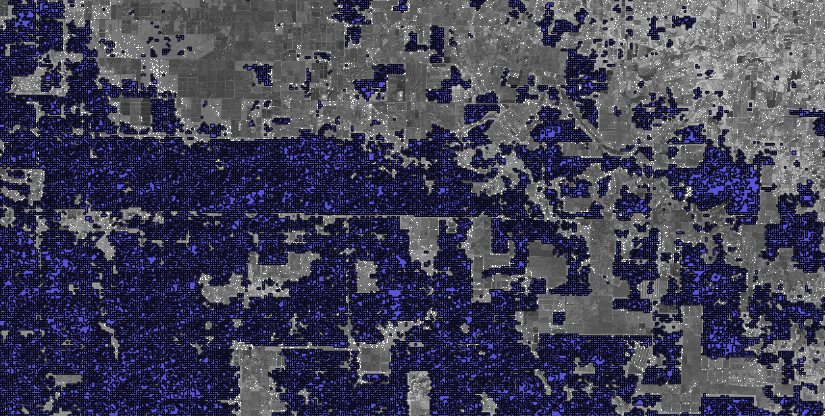
\includegraphics[width=0.8	\textwidth]{./Figures/cap5/mascaraVCF.png}
	\caption{Mascara VCF de 0-30\% sobre NDVI a\~{n}o 2000}
	\label{fig:mascVCf}
\end{figure}
En la Figura \ref{fig:aleatorioVCf} podemos observar parte de los 2000 puntos aleatorios extra\'idos de la mascara VCF (0\%-30\%) para ser cruzados con los niveles digitales de las im\'agenes NDVI.
\begin{figure}[H]
	\centering
	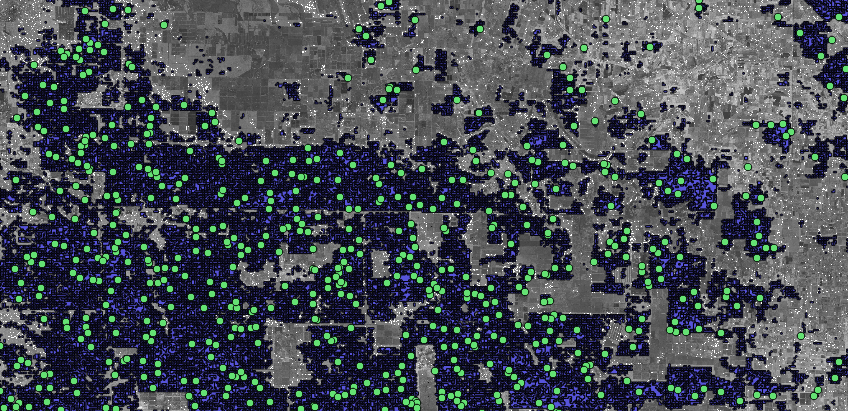
\includegraphics[width=0.8	\textwidth]{./Figures/cap5/vcfAleatorio.png}
	\caption{Puntos aleatorios dentro de la mascara VCF.}
	\label{fig:aleatorioVCf}
\end{figure}
El procedimiento se repite para cada mascara en los distintos rangos. En total se obtiene 5 grupos por cada a\~{n}o estudiado con estad\'isticas ilustrada en la Tabla \ref{t:vcfNdvi}.

% Please add the following required packages to your document preamble:
% \usepackage[table,xcdraw]{xcolor}
% If you use beamer only pass "xcolor=table" option, i.e. \documentclass[xcolor=table]{beamer}
\begin{table}[H]
	\centering
	\begin{tabular}{|l|l|l|}
		\hline
		\rowcolor[HTML]{EFEFEF} 
		\multicolumn{3}{|c|}{\cellcolor[HTML]{EFEFEF}\textbf{A\~{n}o 1986}}        \\ \hline
		\rowcolor[HTML]{EFEFEF} 
		\textbf{VCF (\%)} & \textbf{$ \mu_{ndvi_{ft}} $} & \textbf{$ \sigma_{ndvi_{ft}} $} \\ \hline
		50                & 0.356701              & 0.047891                   \\ \hline
		40                & 0.344022              & 0.0507296                  \\ \hline
		30                & 0.337696              & 0.061581                   \\ \hline
		20                & 0.339586              & 0.0632055                  \\ \hline
		10                & 0.335528              & 0.0727573                  \\ \hline
		\rowcolor[HTML]{EFEFEF} 
		\multicolumn{3}{|c|}{\cellcolor[HTML]{EFEFEF}\textbf{A\~{n}o 1990}}        \\ \hline
		\rowcolor[HTML]{EFEFEF} 
		\textbf{VCF (\%)} & \textbf{$ \mu_{ndvi_{ft}} $} & \textbf{$ \sigma_{ndvi_{ft}} $} \\ \hline
		50                & 0.278804              & 0.0631834                  \\ \hline
		40                & 0.264651              & 0.0679451                  \\ \hline
		30                & 0.254145              & 0.0742348                  \\ \hline
		20                & 0.252186              & 0.0759032                  \\ \hline
		10                & 0.251421              & 0.0796667                  \\ \hline
		\rowcolor[HTML]{EFEFEF} 
		\multicolumn{3}{|c|}{\cellcolor[HTML]{EFEFEF}\textbf{A\~{n}o 1990}}        \\ \hline
		\rowcolor[HTML]{EFEFEF} 
		\textbf{VCF (\%)} & \textbf{$ \mu_{ndvi_{ft}} $} & \textbf{$ \sigma_{ndvi_{ft}} $} \\ \hline
		50                & 0.0202133             & 0.0572825                  \\ \hline
		40                & 0.0104289             & 0.0608757                  \\ \hline
		30                & -0.00337075           & 0.066776                   \\ \hline
		20                & -0.00663188           & 0.0695777                  \\ \hline
		10                & -0.0103891            & 0.0757546                  \\ \hline
	\end{tabular}
		\caption{Media y desviaci\'on del muestreo realizado.}
		\label{t:vcfNdvi}
\end{table}

La Tabla \ref{t:vcfNdvi} nos muestra que la media del NDVI es diferente para cada a\~{n}o, independientemente del porcentaje de vegetaci\'on evaluado, debido a que el \'area foliar (hojas) en la vegetaci\'on posee diferente respuesta espectral para cada especie y \'epoca en la que es capturada por los sensores remotos. En este caso, no es conveniente tomar la media ($  \mu_{ndvi_{ft}} $) dentro de un patr\'on de comportamiento con el fin de discriminar la vegetaci\'on. Las desviaciones ($ \sigma_{ndvi_{ft}} $) se observan pr\'oximas para cada evaluaci\'on por lo que consideramos resaltante y \'util para la discriminaci\'on forestal. Un promedio entre todas las desviaciones es realizado quedando como variable $ \sigma_{c} $ en la umbralizaci\'on de vegetaci\'on  $ \sigma_{c} = 0.0658242733 $.
\subsection{Estimaci\'on de p\'erdida de carbono forestal}\label{subsec:estimacionCarbono}
El Mapa Global de Carbono nos permite analizar una relaci\'on posible con los indices de vegetaci\'on. Los NDVI fueron calculados a partir de im\'agenes Landsat del a\~{n}o 2003, debido a que el Mapa Global de Carbono corresponde a la d\'ecada del a\~{n}o 2000 (como se hab\'ia comentado en la secci\'on \ref{sec:saatchiMapa}). Posteriormente se generaron 240 puntos aleatorios dentro \'areas que correspond\'ian a vegetaci\'on como podemos observar en la Figura \ref{fig:aleatorioCrb}.
\begin{figure}[H]
	\centering
	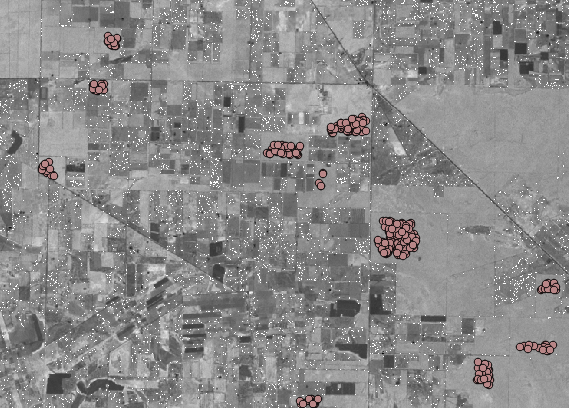
\includegraphics[width=0.8	\textwidth]{./Figures/cap5/carbNdvi.png}
	\caption{Puntos aleatorios.}
	\label{fig:aleatorioCrb}
\end{figure}
Estos puntos fueron generados para interceptar en ellos los NDVI y ton C/ha en el espacio geográfico. De esa manera nos permiti\'o realizar un an\'alisis de regresi\'on lineal, como podemos ver en la Figura \ref{fig:linealCar}, donde el coeficiente de determinaci\'on fue moderado ($ r^{2}=0.509125 $), .
\begin{figure}[H]
	\centering
	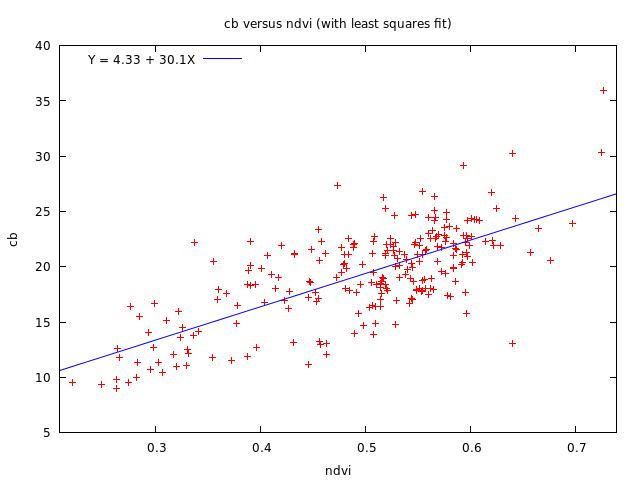
\includegraphics[width=0.8	\textwidth]{./Figures/cap4/ndviCarb.png}
	\caption{Regresi\'on Lineal. $ X=NDVI, Y=TonC/ha $}
	\label{fig:linealCar}
\end{figure}
Los coeficientes de la ecuaci\'on \ref{ec:regreLinelCarb} encontrados en el experimento corresponden a $ m=30.1 $ y $ h =4,33 $, quedando la ecuaci\'on con la siguiente expresi\'on:
\begin{equation}\label{ec:regreLinelCarbExp}
C(x,y)=4.33+30.1 \times ndvi_{f}(x,y)
\end{equation}
La ecuaci\'on \ref{ec:carbonoFinalm} determinada en base a la imagen de \'indice de cambio $ I_{c} $ queda con la siguiente expresi\'on una vez remplazado el coeficiente $ m $:
 \begin{equation}\label{ec:carbonoFinalmExp}
 PC(x,y) = 2.709 \times Ic(x,y)
 \end{equation}


\subsection{Prueba experimental} 
Con el prop\'osito de evaluar la calidad en la detecci\'on de cambio, se obtuvieron las im\'agenes que fueron utilizadas en la elaboraci\'on del Paraguay Forest Change Product (secci\'on \ref{sec:fcc}). Dichas im\'agenes corresponden a la fecha 1-26-1992	del sat\'elite Landsat-5 y 8-17-1999 del satelite Landsat-7, con path-row 228-76 del WRS-2 cubriendo al \'area del caso de estudio.\\~\\
Sectores fueron delimitados en base al uso del suelo empleado en dicha \'area. Esto es con el fin de evaluar la detecci\'on en diferentes condiciones:
\begin{itemize}
	\item \textbf{\'Area Urbana:} zona de aglomeramiento y mayor densidad poblacional. Existe predominio  de actividades econ\'omicas no agropecuarias, sumado a la poblaci\'on total. 
	\item \textbf{\'Area Rural:} se caracteriza por la inmensidad de espacios verdes que la componen y que por esta razón est\'a destinada y es utilizada para la realizaci\'on de actividades agropecuarias y agro-industriales.
	\item \textbf{\'Area H\'umeda:}	zona de tierras, generalmente planas, cuya superficie se inunda de manera permanente o intermitente.
\end{itemize}
En la Figura \ref{fig:zonasEva} podemos observar las \'areas seleccionadas dentro de la imagen satelital. El \'area urbana contiene a la zona c\'entrica del distrito de Filadelfia mientras que el \'area rural a zonas retiradas donde la vegetaci\'on es predominante. Las \'areas h\'umedas corresponden a zonas cercanas al rio Pilcomayo, donde las inundaciones a causa de subidas del rio son frecuente.   
\begin{figure}[H]
	\centering
	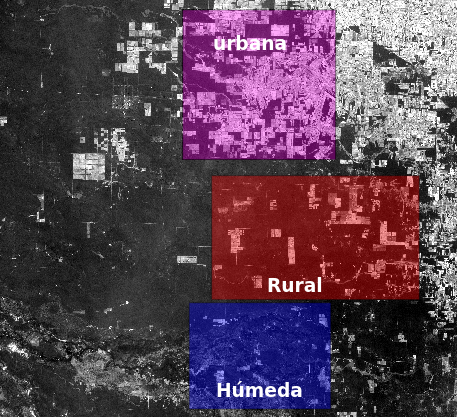
\includegraphics[width=0.7	\textwidth]{./Figures/cap5/zonas.png}
	\caption{\'Areas de los sectores empleados para los experimentos.}
	\label{fig:zonasEva}
\end{figure}
En la Tabla \ref{t:poligonos} podemos observar las coordenadas de los pol\'igonos (xMax,yMax,xMin,yMin) con su per\'imetro (Km) y \'area (Has.) correspondiente a cada sector elegido, de manera a brindar mayores detalles para su reproducci\'on.
\begin{table}[H]
	\centering
	\begin{tabular}{|l|l|l|l|l|l|l|}
		\hline
		\rowcolor[HTML]{EFEFEF} 
		\textbf{Sector} & \textbf{xMin} & \textbf{yMin} & \textbf{xMax} & \textbf{yMax} & \textbf{Has.} & \textbf{Km.} \\ \hline
		Urbano          & 748797.48     & -2532113.76   & 799869.96     & -2482116.50 & 255348.41 & 202.13   \\ \hline
		Rural           & 758474.37     & -2578885.40   & 827825.42     & -2537489.81 & 287082.72 & 221.49  \\ \hline
		Húmedo          & 750947.90     & -2615442.54   & 798257.14     & -2579960.61 & 167862.32 & 165.58	  \\ \hline
	\end{tabular}
		\caption{Pol\'igono de las \'areas. Sistema de coordenadas UTM Zona 20 K. }
		\label{t:poligonos}
\end{table}
El proceso de correcci\'on de las im\'agenes satelitales (secci\'on \ref{sec:correcionesImages}), debido a que obtuvieron los productos L1T del USGS (secci\'on \ref{sec:landsat}), no fueron implementados por ya poseer el pre-procesamiento de correcci\'on geom\'etrica y radiom\'etrica correspondiente. Esto es beneficioso al estudio en cuanto a costo, por no ser necesario el levantamiento de los puntos de control (GCP) en el terreno para la correcci\'on geom\'etrica espec\'ificamente.\\~\\
El $ \epsilon $ utilizado para el punto de parada en el proceso de iteraci\'on es de $ 0.01 $.\\~\\
Las im\'agenes satelitales de entrada son de baja resoluci\'on espacial ($ 30 \times 30 $ metros cuadrados) por lo que el tama\~{n}o de ventana a utilizar seria $ 3 \times 3 $ en el filtro de mediana. \\~\\
 La Tabla \ref{t:pathRow} nos muestra los path/row (secci\'on \ref{sec:landsat}) de las im\'agenes utilizadas en nuestro experimento.

% Please add the following required packages to your document preamble:
% \usepackage[table,xcdraw]{xcolor}
% If you use beamer only pass "xcolor=table" option, i.e. \documentclass[xcolor=table]{beamer}
\begin{table}[H]
	\centering

	\begin{tabular}{|l|l|l|}
		\hline
		\rowcolor[HTML]{EFEFEF} 
		\textbf{Sat\'elite} & \textbf{Path-row} & \textbf{Fecha}  \\ \hline
		Landsat-5         & 228-76            & 1-26-199       \\ \hline
		Landsat-7         & 229-76            & 8-17-1999      \\ \hline
	\end{tabular}
		\caption{Path/row de las im\'agenes utilizadas en el experimento.}
		\label{t:pathRow}
\end{table}

Se recortaron las bandas de las im\'agenes, infrarroja cercana y roja, para cada sector y fecha e introducidas como datos de entrada en la metodolog\'ia. Las Figura \ref{fig:ubana} muestra la m\'ascara de perdida forestal ($ MPF $) junto con la cuantificaci\'on de carbono ($ CCP $) en el \'area urbana para cada coeficientes de fiabilidad ($ n $) (secci\'on \ref{sec:umbralEstadistico2}), obtenidos luego de aplicar la metodolog\'ia presentada.
\begin{figure}[H]
	\centering
	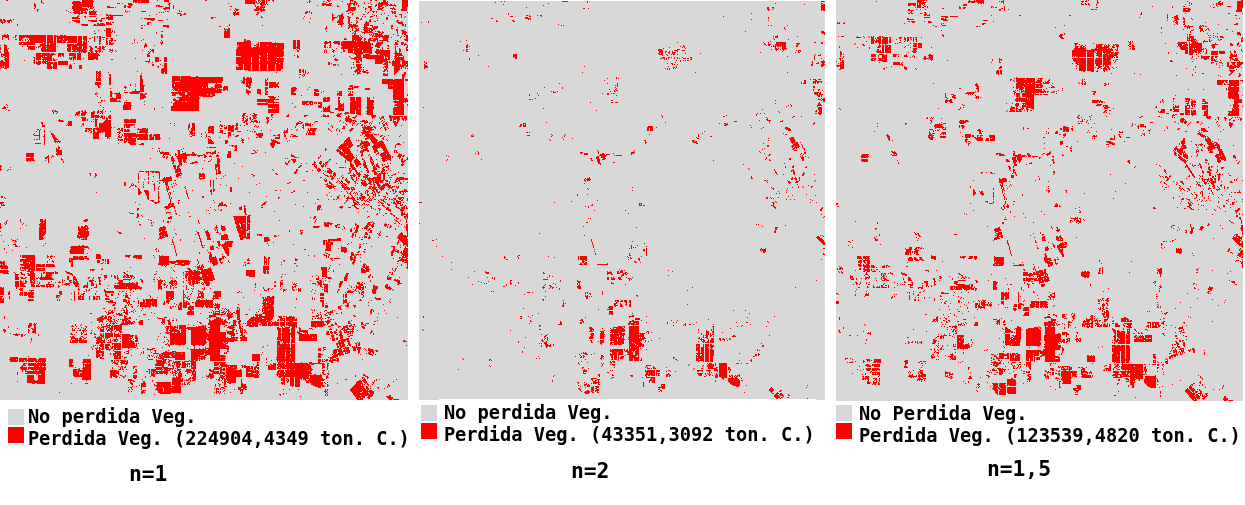
\includegraphics[width=1.0	\textwidth]{./Figures/cap5/res_zona_urbana.png}
	\caption{\'Area Urbana. Mapa de perdida forestal y toneladas de carbono perdidos.}
	\label{fig:ubana}
\end{figure}
La Figura \ref{fig:rural} muestra la m\'ascara de perdida forestal ($ MPF $) junto con la cuantificaci\'on de carbono ($ CCP $) en el \'area rural para cada coeficientes de fiabilidad ($ n $) (secci\'on \ref{sec:umbralEstadistico2}), obtenidos luego de aplicar la metodolog\'ia presentada. 
\begin{figure}[H]
	\centering
	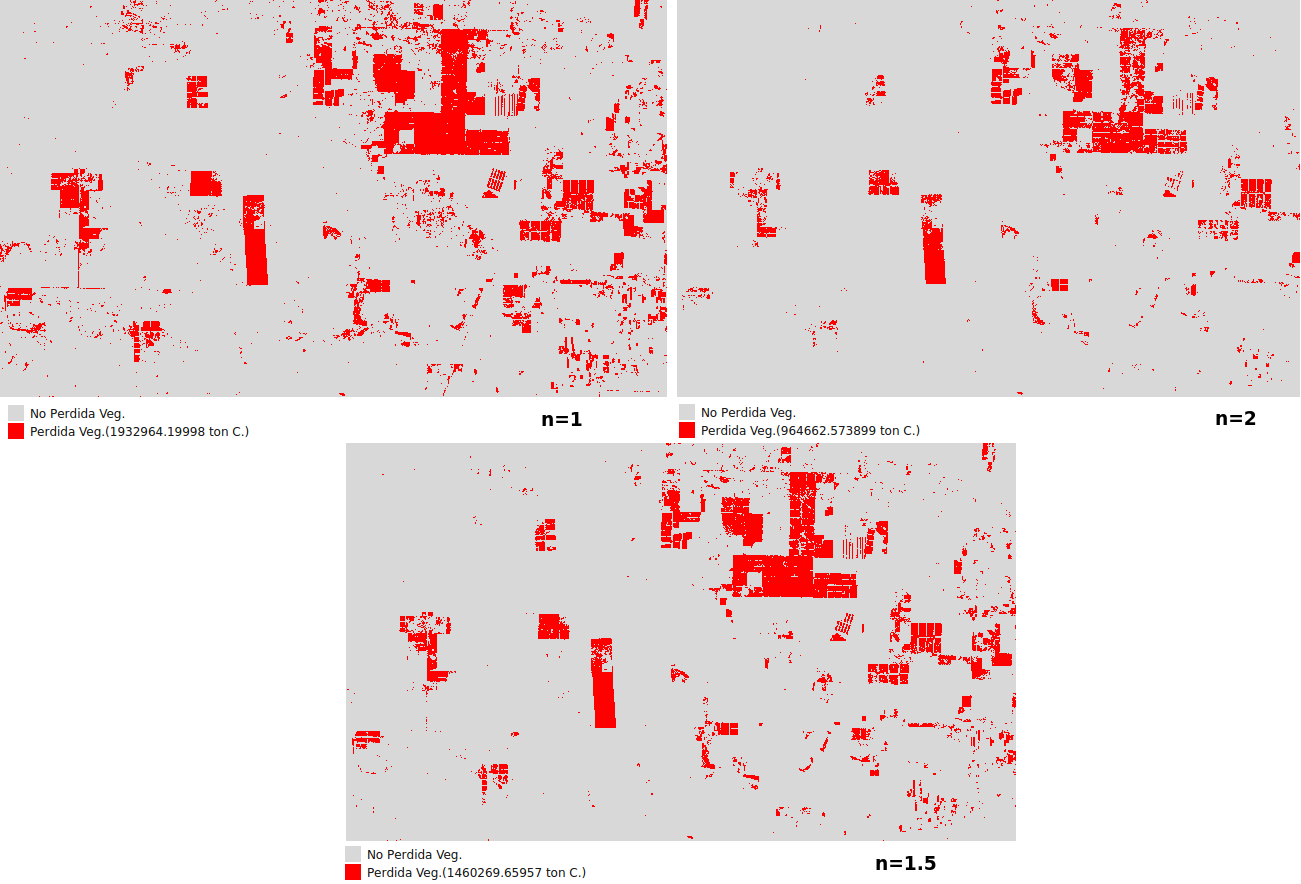
\includegraphics[width=1.0	\textwidth]{./Figures/cap5/res_zona_rural.png}
	\caption{\'Area Rural. Mapa de perdida forestal y toneladas de carbono perdidos}
	\label{fig:rural}
\end{figure}
La Figura \ref{fig:humeda} muestra la m\'ascara de perdida forestal ($ MPF $) junto con la cuantificaci\'on de carbono ($ CCP $) en el \'area h\'umeda para cada coeficientes de fiabilidad ($ n $) (secci\'on \ref{sec:umbralEstadistico2}), obtenidos luego de aplicar la metodolog\'ia presentada.
\begin{figure}[H]
	\centering
	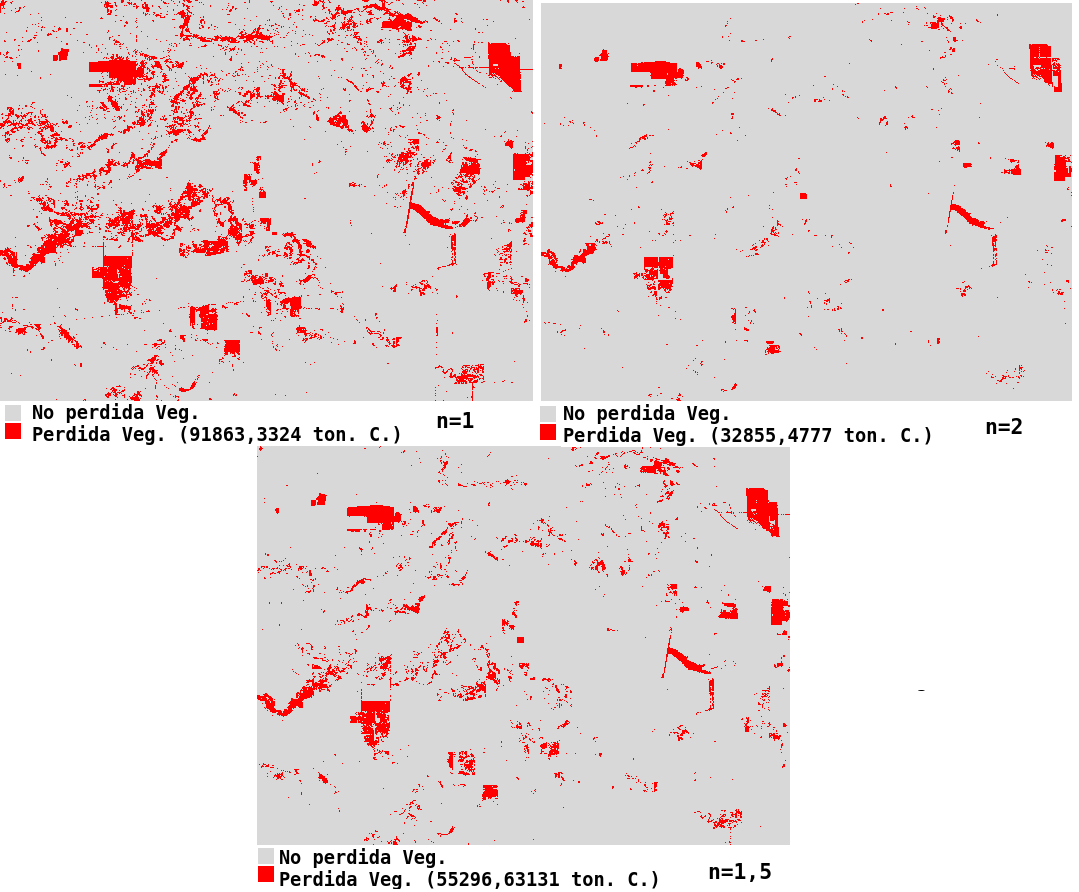
\includegraphics[width=1.0	\textwidth]{./Figures/cap5/res_zona_humeda.png}
	\caption{\'Area H\'umeda. Mapa de perdida forestal y toneladas de carbono perdidos}
	\label{fig:humeda}
\end{figure}


La evaluaci\'on de la calidad en la detecci\'on de perdida forestal ($ MP $) fueron hechas con la comparaci\'on del Paraguay Forest Change Produc (PFCP) y los resultados obtenidos por cada sector y coeficiente de tolerancia $ (n) $. El indice kappa y la precisi\'on global nos permiti\'a saber la calidad en los resultados de detecci\'on de cambio forestal.\\~\\
Una re-clasificaci\'on en la imagen PFCP fue realizado previamente, ya que en ella clasifica dos tipos de bosques (Atl\'antico y Chaco), no bosques y agua. La re-clasificaci\'on consisti\'o en dejar solo los pixeles que representan perdida de vegetaci\'on en cualquier de los tipos, generando una imagen binaria (rojo para pixeles con perdida forestal y amarillo otros) como podemos observar en la Figura \ref{fig:pfcp}.
\begin{figure}[H]
	\centering
	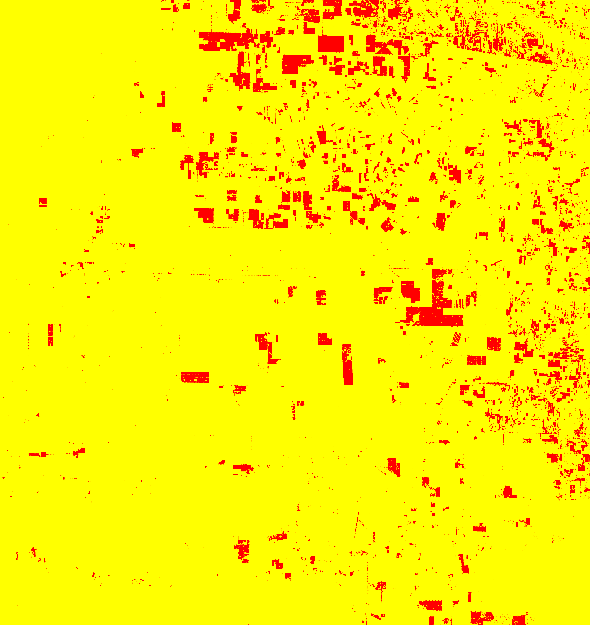
\includegraphics[width=0.4	\textwidth]{./Figures/cap5/pcfp.png}
	\caption{Re-clasificaci\'on de la imagen PFCP. Perdida = 1, Otros=0}
	\label{fig:pfcp}
\end{figure}
Una vez generado la imagen de referencia para la evaluaci\'on con ayuda de la aplicaci\'on GRASS GIS se obtuvo los siguientes resultados:
% Please add the following required packages to your document preamble:
% \usepackage[table,xcdraw]{xcolor}
% If you use beamer only pass "xcolor=table" option, i.e. \documentclass[xcolor=table]{beamer}
\begin{table}[H]
	\centering

	\begin{tabular}{|l|l|l|}
		\hline
		\rowcolor[HTML]{EFEFEF} 
		\multicolumn{3}{|l|}{\cellcolor[HTML]{EFEFEF}\textbf{N=1}}   \\ \hline
		\rowcolor[HTML]{EFEFEF} 
		\textbf{\'Area}  & \textbf{Kappa}  & \textbf{Precisi\'on Global} \\ \hline
		Urbano         & 0.476389        & 84.257452                 \\ \hline
		Rural          & 0.65782         & 93.82121                  \\ \hline
		H\'umeda         & 0.301541        & 90.624794                 \\ \hline
		\rowcolor[HTML]{EFEFEF} 
		\multicolumn{3}{|l|}{\cellcolor[HTML]{EFEFEF}\textbf{N=1.5}} \\ \hline
		\rowcolor[HTML]{EFEFEF} 
		\textbf{\'Area}  & \textbf{Kappa}  & \textbf{Precisi\'on Global} \\ \hline
		Urbano         & 0.315273        & 83.514875                 \\ \hline
		Rural          & 0.671753        & 94.899171                 \\ \hline
		H\'umeda         & 0.425555        & 96.693648                 \\ \hline
		\rowcolor[HTML]{EFEFEF} 
		\multicolumn{3}{|l|}{\cellcolor[HTML]{EFEFEF}\textbf{N=2}}   \\ \hline
		\rowcolor[HTML]{EFEFEF} 
		\textbf{\'Area}  & \textbf{Kappa}  & \textbf{Precisi\'on Global} \\ \hline
		Urbano         & 0.09368         & 81.642457                 \\ \hline
		Rural          & 0.570687        & 94.33648                  \\ \hline
		H\'umeda         & 0.425555        & 96.693648                 \\ \hline
	\end{tabular}
		\caption{Coeficiente Kappa y precisi\'on Global obtenidos.}
		\label{t:kappaGa}
\end{table}

En la Figura \ref{fig:kappaGrafico} podemos observar que los coeficientes kappas en todos los $ n  $ son mejores para zonas rurales, variando en resultados moderados y considerables. Las zonas h\'umedas, donde $ n=1 $ se obtienen resultados aceptables a diferencia de las dem\'as que son moderadas. Por ultimo las zonas urbanos son las que presentan gran variaci\'on entre los coeficientes hallados para el, debiendo implementar tolerancia baja $(n=1)$, al modelo de detecci\'on, para obtener resultados moderados. Los coeficientes son interpretados seg\'un la Tabla \ref{t:kappaTable}.
\begin{figure}[H]
	\centering
	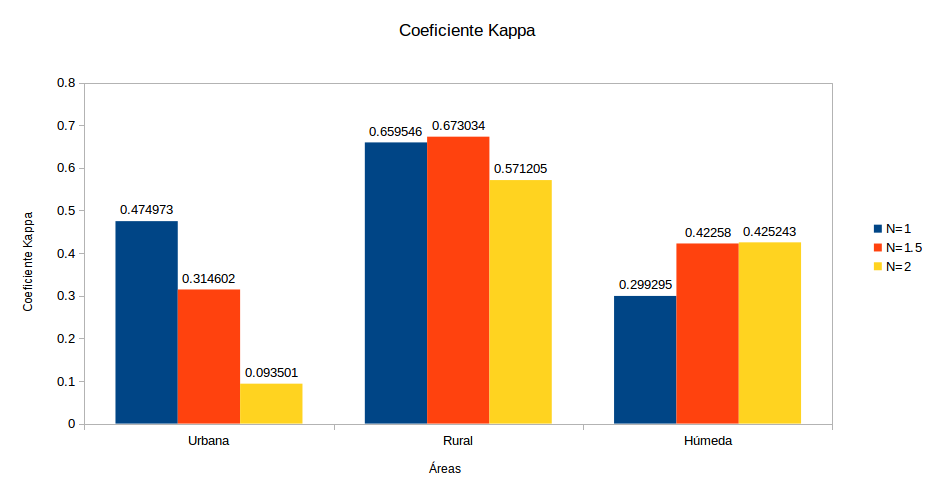
\includegraphics[width=0.8	\textwidth]{./Figures/cap5/kappaGrafico.png}
	\caption{Coeficiente Kappa por cada \'Area y tolerancia.}
	\label{fig:kappaGrafico}
\end{figure}
La precisi\'on global, seg\'un la ilustraci\'on \ref{fig:gaGrafico}, nos dice que el mejor resultado fue en la zona h\'umeda $ (n=2) $ bajando el porcentaje para los dem\'as tolerancias. Pero en zonas rurales obtenemos porcentajes parejos y elevados para cualquier $ n $. Tanto para zonas h\'umedas y rurales seg\'un Jensen \cite{jensen1981urban} son \'optimos por sobrepasar el 85\%. Las zonas urbanas se encuentran entre 81\% - 85\% proximos al umbral, lo que los deja sin ning\'un resultado satisfactorio.
\begin{figure}[H]
	\centering
	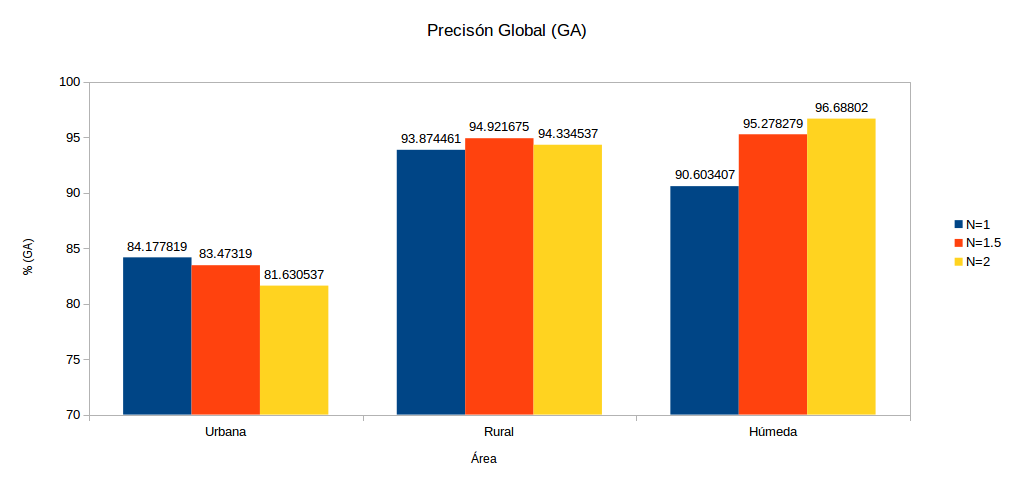
\includegraphics[width=0.8	\textwidth]{./Figures/cap5/gaGrafico.png}
	\caption{GA por cada \'Area y tolerancia.}
	\label{fig:gaGrafico}
\end{figure}
\subsection{Dificultades encontradas} 
Unas de las principales dificultades encontradas fue de que las im\'agenes Landsat presentan un porcentaje de nubosidad en algunas fechas, por lo que requerir\'a de un pre-procesamiento que permita su utilizaci\'on en el an\'alisis. Las correcciones geom\'etricas constituyen un problema adicional si no se utilizan las im\'agenes Lansadt del USGS (secci\'on \ref{sec:landsat}), ya que necesitaran de un previo trabajo de campo para el relevamiento de puntos de control necesarios en la correcci\'on.\\~\\
Los resultados evaluados en base a los objetivos propuestos, en el siguiente y \'ultimo cap\'itulo se exponen las conclusiones de este trabajo  y finalmente trabajos futuros que puedan dar continuidad a este trabajo final de grado.
\subsection{Discusi\'on de resultados}
Una vez evaluado las diferentes zonas de nuestro caso de estudio, podemos darnos cuenta que la metodolog\'ia propuesta posee una mejor respuesta, respecto a la calidad, en \'areas rurales. Esto es debido a que el Coeficiente kappa o los indices de acuerdo var\'ian entre 0.57-0.67 y su precisi\'on global sobrepasan el umbral optimo de 85\%, para cada coeficiente de tolerancia $ n $. Por lo que se considera satisfactorio la metodolog\'ia propuesta, ya que la perdida de carbono es un fen\'omeno frecuente en \'areas con vegetaci\'on predominante.\\~\\	
Zonas donde la vegetaci\'on no predomina, esta metodolog\'ia podr\'ia no resultar suficientemente conveniente. Las pruebas experimentales hechas en zonas urbanas, la precisi\'on global y el coeficiente kappa no son \'optimos por el cual se llega a esa interpretaci\'on.\\~\\
 En \'areas cercanas a r\'ios o sujetas a inundaci\'on, se observaron resultados aceptables para  estudios con tolerancias medias y altas en la detecci\'on de perdida forestal. El monitoreo en estos tipos de zonas con la metodolog\'ia propuesta podr\'ia ser aun de gran utilidad, ya que la presencia de agua en la vegetaci\'on modifica la respuesta espectral, dificultando su clasificaci\'on como cobertura vegetal.\\~\\	
 Los an\'alisis estad\'isticos empleados tanto para la determinaci\'on de umbrales vegetaci\'on/no vegetaci\'on como en el hallazgo de ecuaciones de transformaci\'on a carbono, nos indica que empleando extracciones de indices vegetales y variables estad\'isticas es posible generar metodolog\'ias no complejas destinadas al monitorio ambiental. Esta sencillez nos libera de necesarias supervisiones y entrenamientos normalmente empleadas en teledetecci\'on.\\~\\	
El mapa global de carbono \cite{saatchi2011benchmark} constituy\'o un factor importante para la automatizaci\'on, al permitir determinar una ecuaci\'on que transforme el indice vegetal a carbono. De no existir, hubiese sido necesario aplicar previos muestreos forestales en el terreno.\\~\\	
 La correcci\'on geom\'etrica implica procesos que engloba visitas al terreno para levantamientos de puntos de control requeridas en las interpolaciones. Gracias a la utilizaci\'on de im\'agenes Landsat L1T prove\'idas por la USGS, no fue necesario sumar ese costo a la metodolog\'ia.
